\section{Renormalization}
\subsection{Review of the One-Loop Integral Calculation}
Last time, we studied the computation of the one loop integral $\Gamma_I(k_1, k_2, k_3, k_4)$:

\begin{center}
    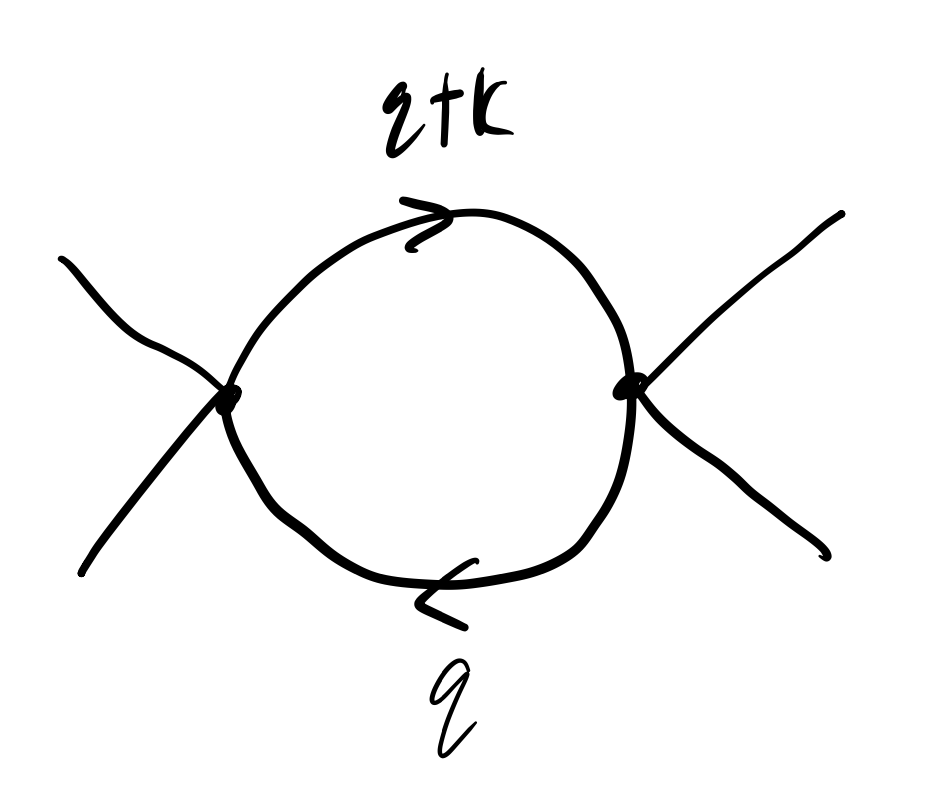
\includegraphics[scale=0.5]{Images/fig-lec29feynman1.png}
\end{center}

These integrals are generally tabulated in the literature, but it is instructive to go through it - they form the backbone of QFT calculations. Let us review it briefly. It is order two in the coupling, so we have a factor of $(-i\lambda)^2$. We then did the combinatorics, to find that we had a factor of $\frac{1}{2}$. The sophisticated Feynman diagrammers would tell you that this two is just the order of the discrete symmetries in this diagram. Going to the irreducible diagram we have to the general diagrams (Which can be reducible), all we do is attatch two-point functions on the external legs, e.g.

\begin{center}
    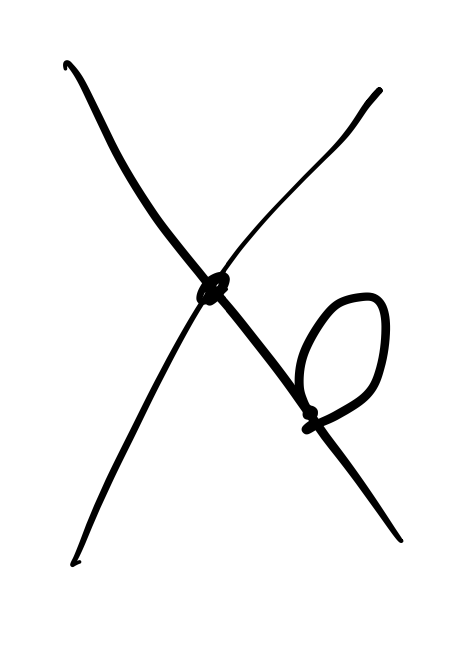
\includegraphics[scale=0.5]{Images/fig-lec29feynman2.png}
\end{center}

and this yields the correct combinatorics, and the reason why we know this formally is because we can go back to the generating functional, take 4 functional derivatives, do the combinatorics, and see that it indeed works out. We had an integral over the loop momentum (recall - one integral per closed loop in the diagram):
\begin{equation}
    \frac{(-i\lambda)^2}{2}\int \frac{d^4q}{(2\pi)^4}\frac{-i}{q^2 + m^2 - i\e}\frac{-i}{(q+k)^2 + m^2 - i\e}
\end{equation}
we then took on the task of actually doing this integral. We started by doing regularization, specifically via dimensional regularization:
\begin{equation}
    \frac{\lambda^2}{2}\mu^{4 - 2w}\int \frac{d^{2w}q}{(2\pi)^{2w}}\frac{1}{q^2 + m^2 - i\e}\frac{1}{(q+k)^2 + m^2 - i\e}
\end{equation}
where we introduce $\mu$ to keep the dimension of the integral consistent. We could then use Wick rotation/Feynman parameters; Wick rotation replaces $q_0 \to iq_0$ and $k_0 \to ik_0$ which makes the metric positive and Euclidean, and the integral becomes over real variables! We then introduce Feynman parameters:
\begin{equation}
    \frac{1}{AB} = \int_0^1 d\alpha \frac{1}{(\alpha A + (1 - \alpha)B)^2}
\end{equation}
so then our integral becomes:
\begin{equation}
    \frac{i\lambda^2}{2}\int_0^1 d\alpha \mu^{4-2w}\int \frac{dq^{2w}}{(2\pi)^{2w}}\frac{1}{(q^2 + \alpha(1-\alpha)k^2 + m^2)^2}
\end{equation}
which is a nice way of phrasing it as it preserves the symmetry (here, Euclidean rotational symmetry, after doing the Wick rotation). 

\subsection{Computing the Dimensionally Regularized Integral}
How do we do integrals that look like:
\begin{equation}
    \int \frac{d^{2w}q}{(2\pi)^{2w}}\frac{1}{(q^2 + m^2)^2}
\end{equation}
If we recall the Gamma function:
\begin{equation}
    \Gamma(s) = \int_0^\infty dx x^{s-1}e^x = \frac{1}{\alpha^s}\int_0^\infty dx x^{s-1}e^{x/\alpha}
\end{equation}
so then:
\begin{equation}
    \begin{split}
        \int \frac{d^{2w}q}{(2\pi)^{w}}\frac{1}{(q^2 + m^2)^2} &= \frac{1}{\Gamma(2)}\int_0^\infty dx x\int e^{-x(q^2 + m^2)} \frac{d^{2w}q}{(2\pi)^{2w}}
        \\ &= \frac{1}{\Gamma(2)}\int_0^\infty dx x e^{-xm^2}\left(\int \frac{d^2q}{(2\pi)^2} e^{-q^2 x}\right)^w
        \\ &= \frac{1}{\Gamma(2)}\int_0^\infty dx x e^{-x m^2}\frac{1}{(4\pi)^w}\frac{q}{x^w}
        \\ &= \frac{\Gamma(2-w)}{(4\pi)^w \Gamma(2)}\frac{1}{(m^2)^{2-w}}
    \end{split}
\end{equation}
and there's our result! There is a slightly more general procedure for this in the textbook, but this is basically it. Going back to our one-loop integral, we therefore conclude:
\begin{equation}
    \frac{i\lambda^2}{2}\int_0^1d\alpha \frac{\Gamma(2-w)}{(4\pi)^w \Gamma(2)}\left(\frac{\mu^2}{M^2}\right)^{2-w}
\end{equation}
where $M^2$ is shorthand. This integral can be evaluated, but it gives some hypergeometric function which is not particularly enlightening, so we leave it as is. The only place where this diverges is for every even dimension $w \geq 4$. What we want to do is an asymptotic expansion in 4 dimensions; to this end:
\begin{equation}
    \Gamma(2 - w) = \frac{1}{2-w} + \gamma + O(2-w)
\end{equation}
where $\gamma$ is the Euler-Mascheroni constant, and $O(2-w) \to 0$ as $w \to 2$. Therefore returning to our integral:
\begin{equation}
    \begin{split}
        &i\frac{\lambda^2}{2}\int_0^1 d\alpha \frac{1}{(4\pi)^2}\left(\frac{1}{2- w} - \gamma\right) \left(1 + (2 - w)\ln \frac{4\pi \mu^2}{M^2}\right) 
        \\ &= \frac{i\lambda^2}{32\pi^2}\frac{1}{2-w} + \frac{i\lambda^2}{32\pi^2}\int_0^1 d\alpha \ln(\frac{4\pi \mu^2 e^{-\gamma}}{\alpha(1-\alpha)k^2 + m^2})
    \end{split}
\end{equation}
We get a singularity coming from kinematics when the reaction can produce real particles as well as virutal particles. There are handwavey explanations for this; virtual particles have no choice but to recombine, but real particles have the option to fly away and become real particles. So we have competing processes of real/virtual particles, and then the unitarity of time evolution tells us that there is an imaginary part of the diagram, which corresponds to the cut singularity of the log\dots

If we stay in the Euclidean regime (rather than going into Minkowski) where $k^2 > 0$, we do not have to worry about this. Som there's our result for this particular Feynman diagram! There were more Feynman diagrams then this one that contributed to the two-point function, which had to do with how the legs were attatched:

\begin{center}
    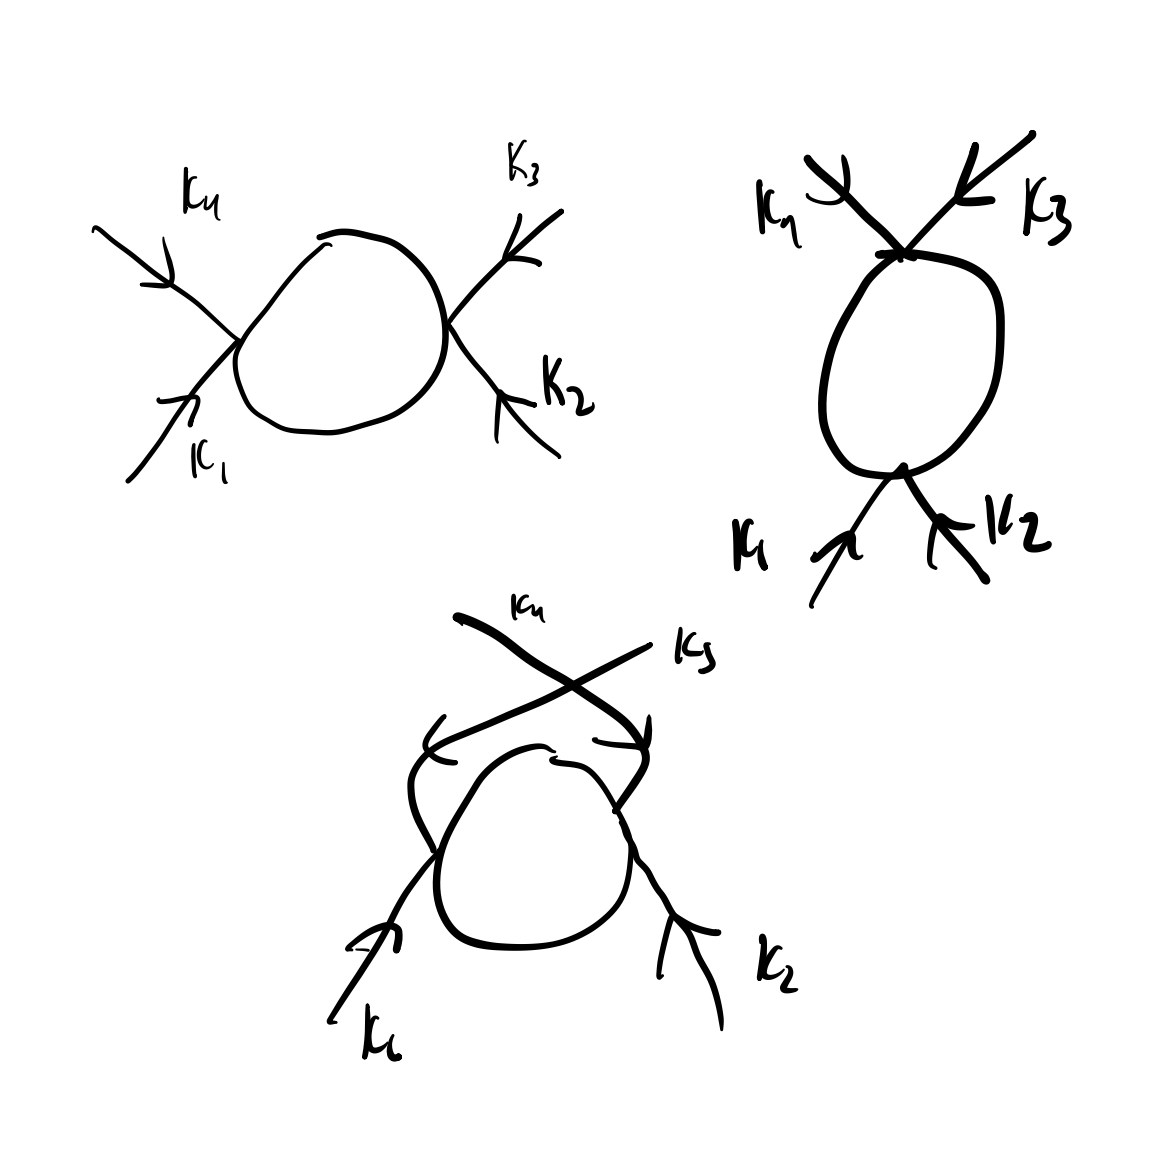
\includegraphics[scale=0.5]{Images/fig-lec29feynman3.png}
\end{center}

Summing over these is imposing bose symmetry, i.e. it should not matter how we permute the momenta. So then summing this with the lower order ($-i\lambda$) term of:
\begin{center}
    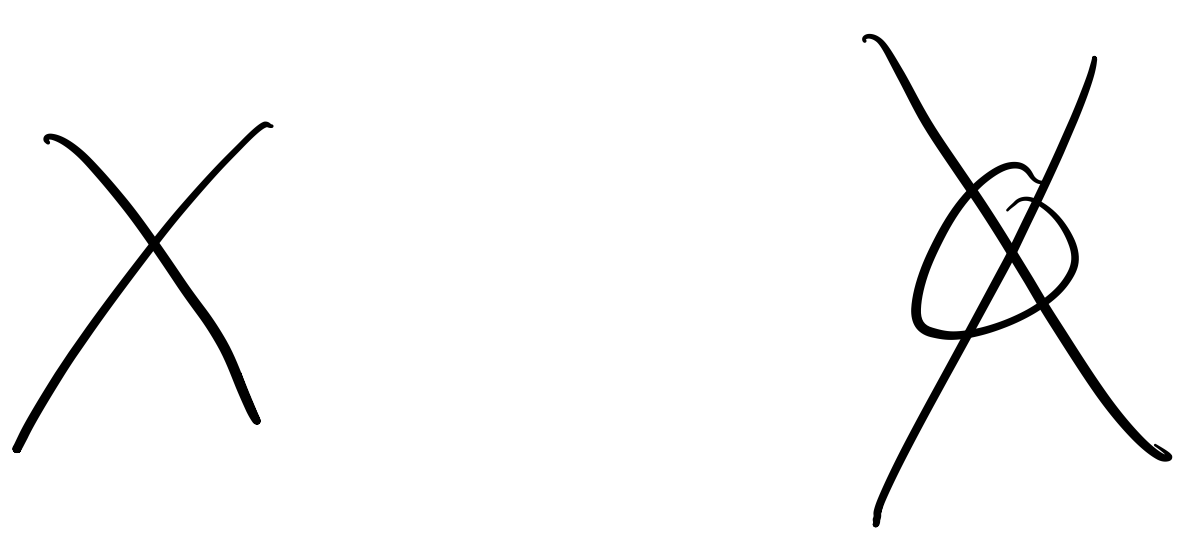
\includegraphics[scale=0.5]{Images/fig-lec29feynman4.png}
\end{center}
as well as the counterterm of $-i\lambda^2 z^{(1)}_\lambda$, we are done!

So in conclusion:
\begin{equation}
    \begin{split}
        \Gamma_I(k_1, k_2, k_3, k_4) &= -i\lambda - i\lambda^2 z_\lambda^{(1)} + \frac{3i\lambda^2}{32\pi^2}\frac{1}{2-w} 
        \\ &+ \frac{i\lambda^2}{32\pi^2}\int_0^1 d\alpha \left(\ln\frac{4\pi \mu^2 e^{-\gamma}}{\alpha(1-\alpha)(k_1 + k_4)^2 + m^2} + \ln\frac{4\pi \mu^2 e^{-\gamma}}{\alpha(1-\alpha)(k_1 + k_2)^2 + m^2} + \ln\frac{4\pi \mu^2 e^{-\gamma}}{\alpha(1-\alpha)(k_1 + k_3)^2 + m^2}\right) 
        \\ &+ O(\lambda^3)
    \end{split}
\end{equation}
Let us to the same order compute the two-point function, and then deal with the counterterm- its role will be to cancel out the singularity.

\subsection{Computing the Two-Point function}
Recall:
\begin{center}
    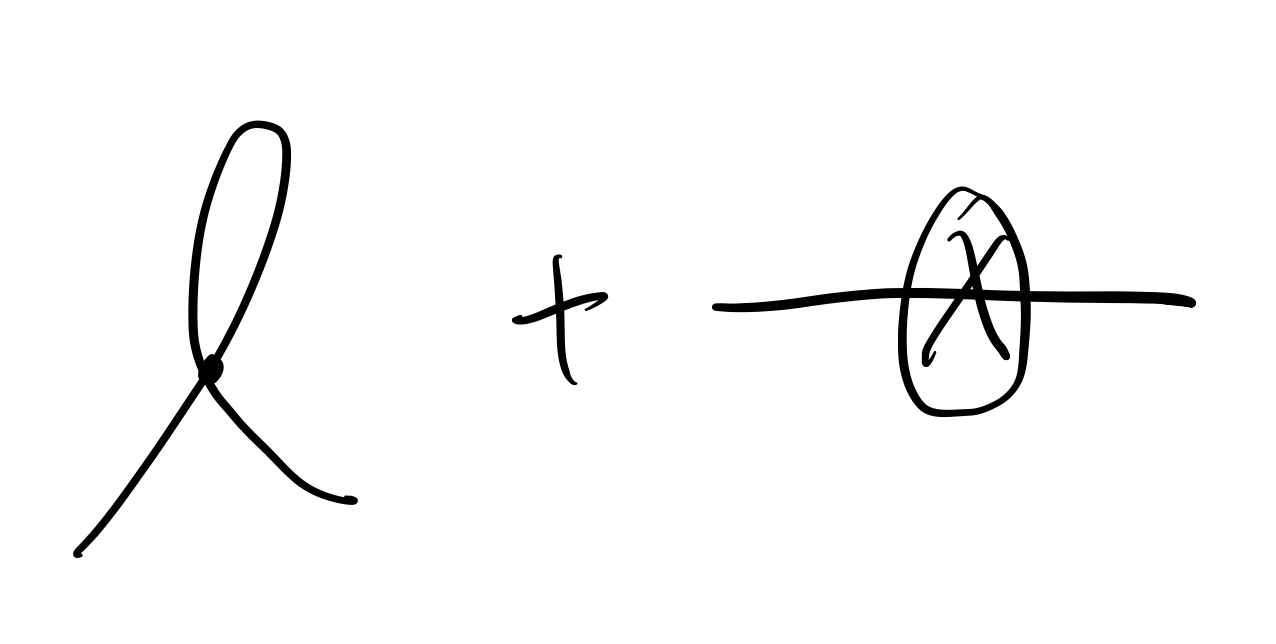
\includegraphics[scale=0.5]{Images/fig-lec29feynman5.png}
\end{center}
which corresponds to:
\begin{equation}
    \Pi(k^2) = -\frac{i\lambda}{2}\int \frac{d^4q}{(2\pi)^4} \frac{-i}{q^2 + m^2 - i\e} - i\lambda \left(z^{(1)}k^2 + z^{(1)}_m m^2\right)
\end{equation}
We need to integrate this; its a bit easier than the previous integral. Dimensionally regularize, put $q_0 \to iq_0$, and use the dimensional regularization formula. We then obtain:
\begin{equation}
    \Pi(k^2) = -\frac{i\lambda}{2}\frac{\Gamma(1 - w)}{(4\pi)^w \Gamma(1)}m^2\left(\frac{m^2}{\mu^2}\right)^{w-2} - i\lambda\left(z^{(1)}k^2 + z^{(1)}_m m^2\right)
\end{equation}
Again one can expand this asymptotically around $w = 2$. Note that $\Gamma(1 - w)$ has a pole there. This yields:
\begin{equation}
    \Pi(k^2) =  \frac{i\lambda}{32\pi^2}m^2\frac{1}{1-w} - \frac{i\lambda_m}{32\pi^2}\ln\frac{m^2}{4\pi \mu^2 e^{1+\gamma}} - i\lambda\left(z^{(1)}k^2 + z^{(1)}_m m^2\right)
\end{equation}
We now should fit the counterterms to observable physics - i.e. to cancel out the infinities, as two-point functions (observables) should not be infinite! Then there are the finite parts of the counterterms, which are determined by \emph{schemes}. There are three popular ones; one is to choose the scheme so that the two-point function still has a singularity at $k^2 = -m^2$. The idea there is to choose the $z$s such that the singularity persists. It is easy to do here; the first term is $k$ independent, so we can choose $z^{(1)} = 0$ and we can then select $z^{(1)}_m$ to cancel out the remaining things, so we reduce things to the propogator. This is what is known as ``on-shell subtraction'', as it places the singularity at the physical mass, preserving the analytic structure.

We need a criterion for $\Gamma_1(k_1, k_2, k_3, k_4)$ as well. We could simply say that for the four particles at rest (the same momentum/$k_i$s), we say that that should be the physical coupling we call $\lambda$, and then choose $z_\lambda^{(1)}$ to cancel everything else when we plug in those momenta into the rest of the expression. We then get a finite result, no UV divergence, and a prediction - this in fact predicts the cross-section of the scattering of two scalar particles.

There are two other common schemes - one is \emph{minimal subtraction}, where you choose the $z$s to cancel out the singularities. In this case the $m$ appearing is not the actual mass of the particle, it is corrected by other terms. $\lambda$ in this case is also not the physical coupling constant - both the physical mass and coupling constant are functions of $m, \lambda$. The nice thing about this scheme is that the counterterms do not depend on the mass, and $\mu$ as well. They only depend on the coupling constant. There is some techncial advantage in this, which we will see in the next lecture.

Finally, there is a $\overline{MS}$ (MS-bar) scheme. This cancels a singularity, as well as the $4\pi e^{-\gamma}$ (which again is just a constant term). There are other schemes, which we will learn a little about next time.

So, we have renormalized some of the important correlation functions here! We will also see what this is good for - i.e. constructing a scattering matrix. We can also construct the full correlation function from the irreducible correlation function, but this we will find will be unnecessary for calculating the scattering matrix. There's a little bit of magic involved. Before this, we will finish the perturbative calculation, by looking at the renormalization group. This is necessary because in the massless limit, the arguments of the logarithms scale as $\frac{1}{k^2}$ - but in PT we expand in small things, and depending on $k$ this might not be the case. The PT turns out to have kinematical limitations, being only accurate when $k^2 \sim \mu^2$ and the logarithms are ``small''. We can fix this by making use of the fact that the $\mu^2$ is arbitrary - the original theory did not depend on this. We can make use of this fact by scaling $\mu$ along with $k$. 